\section{introduction to the heart and its functions}
%%\label{sec:multicore_architectures}
%%Maybe quotes instead?
The heart. The most iconic organ in the human body, responsible for thousands of bad love songs and poorly made decisions. While in reality, the heart is actually a big muscular pump that powers the entire circulatory system, transporting mainly oxygen, nutrients, hormones and heat throughout the body. 

\subsection{Layers of the Heart Wall}
The heart consists of three layers, the \textit{epicardium}, \textit{myocardium}, and the \textit{endocardium}. 

The outermost layer is called the epicardium. The epicardium is a thin layer of connective tissue [19], and fat that serves as a protection from trauma as well as lubricant for the sorrounding environment. 

The heart is constructed with a special kind of muscle tissue called the myocardium, also referred to as the cardiac muscle. Which makes up the majority of the thickness and mass of the heart. The cardiac muscle is one of the main reasons to why the heart pumps blood. When the cardiac muscle cells receives electrictrial stimulation, it results in a rhytmic contraction and relaxtion phase, that makes the heart beat. A deeper description of the electrophysiological process in the heart can be found in section [X.X]

The endocardium is the innermost layer in the heart wall. bla bla

%%which is one of four tissues that supports, connects or separates different types of organs and tissues in the body [19] FOOTNOTE?

\subsection{Chambers of the Heart}
To get an illustrative perspective of the composition of the heart, it helps think of it as a student apartment that is made up of a left and right unit. The left and right unit are seperated by a wall known as a cardiac septum. Student housings are known to be space saving, so each unit is then subdivided into a upper chamber referred to as the \textit{atrium}, and a lower chamber known as the \textit{ventricle}, as illustrated in [FIGURE X.X]. The right atrium (RA) is above the right ventricle (RV), while the left atrium (LA) sits above the left ventricle (LV). If we were to take our student apartment example even further, the only entrance for getting into the left unit is located in the right atrium. This is a one-way entrance, meaning that students can only enter 
%%[http://www.hopkinsmedicine.org/healthlibrary/conditions/cardiovascular_diseases/anatomy_and_function_of_the_heart_valves_90,P03059/]
%%bilde her!

\begin{figure}[h]
 \centering 
     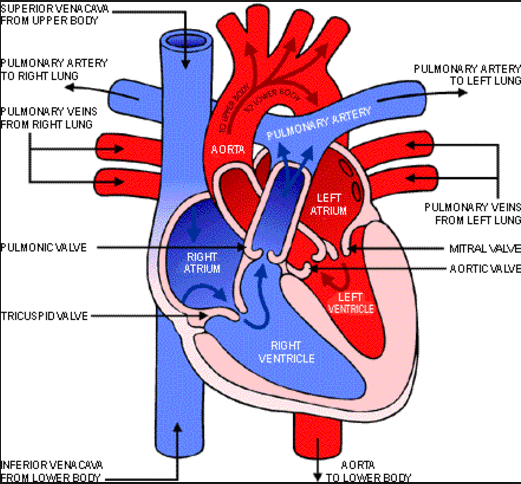
\includegraphics[width=0.9\textwidth]{bilder/b_heart_structure_new}
     \caption{Explaining the decomposition process in a 3 dimensional structured mesh. Illustration taken from \cite{article9}.
     \label{b_heart_structure_new.png}}
\end{figure}

%%the primary function of the cardiovascular system is to supply body cells with nutrient material and carry away waste products
%%, and it does not care about poetry or emotions.

\subsection{The Blood Flow in the Caridovascular System}


%%which came first, the clot or the heart attack?
